\documentclass[aspectratio=169]{beamer}

\usepackage{natbib}

\usetheme{metropolis}           % Use metropolis theme
\title{
    Disentangled Representation Learning for \\
    Stylistic Variation in Neural Language Models}
\date{\today}
\author{Vineet John}
\institute{University of Waterloo}

\begin{document}

\maketitle

\graphicspath{{images/}}

\section{Motivation}

\begin{frame}{Universal Function Approximators}
	\begin{figure}[ht]
		\centering
		\includegraphics[width=\linewidth]{mlp-network}
	\end{figure}
\end{frame}

\begin{frame}{Non-Interpretable Latent Representations}
\end{frame}

\begin{frame}{Problem Statement}
	\centering
	\Huge{Generate plausible sentences in a user-defined style, while retaining the original content of the source sentences.}
\end{frame}

% 

\section{Background}

\begin{frame}{Sequence Autoencoding}
	\centering
	\makeatletter
\ifx\du\undefined
  \newlength{\du}
\fi
\setlength{\du}{\unitlength}
\ifx\spacing\undefined
  \newlength{\spacing}
\fi
\setlength{\spacing}{60\unitlength}
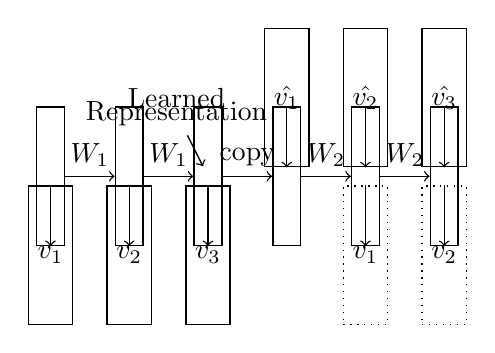
\begin{tikzpicture}
\pgfsetlinewidth{0.5\du}
\pgfsetmiterjoin
\pgfsetbuttcap

\node[rectangle, draw=black, minimum width=10\du, minimum height=50\du] (v1) at (0\spacing, 0) {$v_1$};
\node[rectangle, draw=black, minimum width=10\du, minimum height=50\du] (v2) at (\spacing, 0) {$v_2$};
\node[rectangle, draw=black, minimum width=10\du, minimum height=50\du] (v3) at (2\spacing, 0) {$v_3$};

\node[rectangle, dotted, draw=black, minimum width=10\du, minimum height=50\du] (v5) at (4\spacing, 0) {$v_1$};
\node[rectangle, dotted, draw=black, minimum width=10\du, minimum height=50\du] (v6) at (5\spacing, 0) {$v_2$};

\node[rectangle, draw=black, minimum width=10\du, minimum height=50\du] (h1) at (0\spacing, \spacing) {};
\node[rectangle, draw=black, minimum width=10\du, minimum height=50\du] (h2) at (\spacing, \spacing) {};
\node[rectangle, draw=black, minimum width=10\du, minimum height=50\du] (h3) at (2\spacing, \spacing) {};

\node[rectangle, draw=black, minimum width=10\du, minimum height=50\du] (h4) at (3\spacing, \spacing) {};
\node[rectangle, draw=black, minimum width=10\du, minimum height=50\du] (h5) at (4\spacing, \spacing) {};
\node[rectangle, draw=black, minimum width=10\du, minimum height=50\du] (h6) at (5\spacing, \spacing) {};

\node[rectangle, draw=black, minimum width=10\du, minimum height=50\du] (v4r) at (3\spacing, 2\spacing) {$\hat{v_1}$};
\node[rectangle, draw=black, minimum width=10\du, minimum height=50\du] (v5r) at (4\spacing, 2\spacing) {$\hat{v_2}$};
\node[rectangle, draw=black, minimum width=10\du, minimum height=50\du] (v6r) at (5\spacing, 2\spacing) {$\hat{v_3}$};

\node[anchor=center]  at (1.6\spacing, 2\spacing) {Learned};
\node[anchor=center] (p1) at (1.6\spacing, 1.8\spacing) {Representation};
\node[anchor=center] (p2) at (2\spacing, \spacing) {};
%\node[anchor=center] (w) at (0\spacing, 0.5\spacing) {$\WW_1$};

%\draw[ultra thick, ->] (2aa) -- node[left] {Conv Net} (3a);
\draw[->] (v1) -- (h1);
\draw[->] (v2) -- (h2);
\draw[->] (v3) -- (h3);
\draw[->] (v5) -- (h5);
\draw[->] (v6) -- (h6);

\draw[->] (h1) -- node[above] {$W_1$} (h2);
\draw[->] (h2) -- node[above] {$W_1$} (h3);
\draw[->] (h3) -- node[above] {copy} (h4);
\draw[->] (h4) -- node[above] {$W_2$} (h5);
\draw[->] (h5) -- node[above] {$W_2$} (h6);

\draw[->] (h4) -- (v4r);
\draw[->] (h5) -- (v5r);
\draw[->] (h6) -- (v6r);

\draw[->] (p1) -- (p2);
\end{tikzpicture}


	\tiny{Source: \cite{srivastava2015unsupervised}}
\end{frame}

\begin{frame}{Sequence Autoencoding}
    \textbf{Text Reconstruction}
    Predict next most likely word at each time step
    \begin{equation}
        P(x_1, x_2 \cdots x_t) = \prod_{i=1}^t P(x_i | x_1, \cdots, x_{i-1})
    \end{equation}

    Minimize the negative log-likelihood of each word, given the previous words
\end{frame}

\begin{frame}{Multi-Task Learning}
\end{frame}

\begin{frame}{Adversarial Learning}
\end{frame}

\begin{frame}{Style Transfer}
\end{frame}

\begin{frame}{Style and Content in Language}
\end{frame}

\begin{frame}{Sequence Transduction}
\end{frame}

% 

\section{Approach}

\begin{frame}{Sequence Autoencoder - Deterministic}
\end{frame}

\begin{frame}{Sequence Autoencoder - Variational}
	\citet{kingma2013auto}
\end{frame}

\begin{frame}{Multi-Task Style Classifier}
\end{frame}

\begin{frame}{Style Discriminator}
\end{frame}

\begin{frame}{Content Discriminator}
\end{frame}

% 

\section{Tasks and Datasets}

\begin{frame}{Yelp Service Reviews}
\end{frame}

\begin{frame}{Amazon Product Reviews}
\end{frame}

% 

\section{Evaluation Metrics}

\begin{frame}{Style Transfer Strength}
\end{frame}

\begin{frame}{Content Preservation}
\end{frame}

\begin{frame}{Word Overlap}
\end{frame}

\begin{frame}{Language Fluency}
\end{frame}

% 

\section{Results and Analysis}

\begin{frame}{Latent Space Classification}
\end{frame}

\begin{frame}{Latent Space t-SNE plots}
\end{frame}

\begin{frame}{Style Transfer Results - Yelp}
\end{frame}

\begin{frame}{Style Transfer Results - Amazon}
\end{frame}

% 

\section{Related Work}

\begin{frame}{Controlled Text Generation}
\end{frame}

\begin{frame}{Cross-Aligned Style Transfer}
\end{frame}

\begin{frame}{Style Transfer using Style Embeddings}
\end{frame}

\begin{frame}{Style Transfer using Muliple Decoders}
\end{frame}

% 

\section{Conclusion}

\begin{frame}{Conclusion}
\end{frame}

\begin{frame}[allowframebreaks]
	\bibliographystyle{unsrtnat}
	\bibliography{presentation}
\end{frame}

\begin{frame}
	\centering
	\Huge{Questions?}
\end{frame}


\end{document}
